\documentclass{article} % For LaTeX2e
\usepackage{icomp2024_conference,times}

% Optional math command from https://github.com/goodfeli/dlbook_notation.
%%%%% NEW MATH DEFINITIONS %%%%%

\usepackage{amsmath,amsfonts,bm}

% Mark sections of captions for referring to divisions of figures
\newcommand{\figleft}{{\em (Left)}}
\newcommand{\figcenter}{{\em (Center)}}
\newcommand{\figright}{{\em (Right)}}
\newcommand{\figtop}{{\em (Top)}}
\newcommand{\figbottom}{{\em (Bottom)}}
\newcommand{\captiona}{{\em (a)}}
\newcommand{\captionb}{{\em (b)}}
\newcommand{\captionc}{{\em (c)}}
\newcommand{\captiond}{{\em (d)}}

% Highlight a newly defined term
\newcommand{\newterm}[1]{{\bf #1}}


% Figure reference, lower-case.
\def\figref#1{figure~\ref{#1}}
% Figure reference, capital. For start of sentence
\def\Figref#1{Figure~\ref{#1}}
\def\twofigref#1#2{figures \ref{#1} and \ref{#2}}
\def\quadfigref#1#2#3#4{figures \ref{#1}, \ref{#2}, \ref{#3} and \ref{#4}}
% Section reference, lower-case.
\def\secref#1{section~\ref{#1}}
% Section reference, capital.
\def\Secref#1{Section~\ref{#1}}
% Reference to two sections.
\def\twosecrefs#1#2{sections \ref{#1} and \ref{#2}}
% Reference to three sections.
\def\secrefs#1#2#3{sections \ref{#1}, \ref{#2} and \ref{#3}}
% Reference to an equation, lower-case.
\def\eqref#1{equation~\ref{#1}}
% Reference to an equation, upper case
\def\Eqref#1{Equation~\ref{#1}}
% A raw reference to an equation---avoid using if possible
\def\plaineqref#1{\ref{#1}}
% Reference to a chapter, lower-case.
\def\chapref#1{chapter~\ref{#1}}
% Reference to an equation, upper case.
\def\Chapref#1{Chapter~\ref{#1}}
% Reference to a range of chapters
\def\rangechapref#1#2{chapters\ref{#1}--\ref{#2}}
% Reference to an algorithm, lower-case.
\def\algref#1{algorithm~\ref{#1}}
% Reference to an algorithm, upper case.
\def\Algref#1{Algorithm~\ref{#1}}
\def\twoalgref#1#2{algorithms \ref{#1} and \ref{#2}}
\def\Twoalgref#1#2{Algorithms \ref{#1} and \ref{#2}}
% Reference to a part, lower case
\def\partref#1{part~\ref{#1}}
% Reference to a part, upper case
\def\Partref#1{Part~\ref{#1}}
\def\twopartref#1#2{parts \ref{#1} and \ref{#2}}

\def\ceil#1{\lceil #1 \rceil}
\def\floor#1{\lfloor #1 \rfloor}
\def\1{\bm{1}}
\newcommand{\train}{\mathcal{D}}
\newcommand{\valid}{\mathcal{D_{\mathrm{valid}}}}
\newcommand{\test}{\mathcal{D_{\mathrm{test}}}}

\def\eps{{\epsilon}}


% Random variables
\def\reta{{\textnormal{$\eta$}}}
\def\ra{{\textnormal{a}}}
\def\rb{{\textnormal{b}}}
\def\rc{{\textnormal{c}}}
\def\rd{{\textnormal{d}}}
\def\re{{\textnormal{e}}}
\def\rf{{\textnormal{f}}}
\def\rg{{\textnormal{g}}}
\def\rh{{\textnormal{h}}}
\def\ri{{\textnormal{i}}}
\def\rj{{\textnormal{j}}}
\def\rk{{\textnormal{k}}}
\def\rl{{\textnormal{l}}}
% rm is already a command, just don't name any random variables m
\def\rn{{\textnormal{n}}}
\def\ro{{\textnormal{o}}}
\def\rp{{\textnormal{p}}}
\def\rq{{\textnormal{q}}}
\def\rr{{\textnormal{r}}}
\def\rs{{\textnormal{s}}}
\def\rt{{\textnormal{t}}}
\def\ru{{\textnormal{u}}}
\def\rv{{\textnormal{v}}}
\def\rw{{\textnormal{w}}}
\def\rx{{\textnormal{x}}}
\def\ry{{\textnormal{y}}}
\def\rz{{\textnormal{z}}}

% Random vectors
\def\rvepsilon{{\mathbf{\epsilon}}}
\def\rvtheta{{\mathbf{\theta}}}
\def\rva{{\mathbf{a}}}
\def\rvb{{\mathbf{b}}}
\def\rvc{{\mathbf{c}}}
\def\rvd{{\mathbf{d}}}
\def\rve{{\mathbf{e}}}
\def\rvf{{\mathbf{f}}}
\def\rvg{{\mathbf{g}}}
\def\rvh{{\mathbf{h}}}
\def\rvu{{\mathbf{i}}}
\def\rvj{{\mathbf{j}}}
\def\rvk{{\mathbf{k}}}
\def\rvl{{\mathbf{l}}}
\def\rvm{{\mathbf{m}}}
\def\rvn{{\mathbf{n}}}
\def\rvo{{\mathbf{o}}}
\def\rvp{{\mathbf{p}}}
\def\rvq{{\mathbf{q}}}
\def\rvr{{\mathbf{r}}}
\def\rvs{{\mathbf{s}}}
\def\rvt{{\mathbf{t}}}
\def\rvu{{\mathbf{u}}}
\def\rvv{{\mathbf{v}}}
\def\rvw{{\mathbf{w}}}
\def\rvx{{\mathbf{x}}}
\def\rvy{{\mathbf{y}}}
\def\rvz{{\mathbf{z}}}

% Elements of random vectors
\def\erva{{\textnormal{a}}}
\def\ervb{{\textnormal{b}}}
\def\ervc{{\textnormal{c}}}
\def\ervd{{\textnormal{d}}}
\def\erve{{\textnormal{e}}}
\def\ervf{{\textnormal{f}}}
\def\ervg{{\textnormal{g}}}
\def\ervh{{\textnormal{h}}}
\def\ervi{{\textnormal{i}}}
\def\ervj{{\textnormal{j}}}
\def\ervk{{\textnormal{k}}}
\def\ervl{{\textnormal{l}}}
\def\ervm{{\textnormal{m}}}
\def\ervn{{\textnormal{n}}}
\def\ervo{{\textnormal{o}}}
\def\ervp{{\textnormal{p}}}
\def\ervq{{\textnormal{q}}}
\def\ervr{{\textnormal{r}}}
\def\ervs{{\textnormal{s}}}
\def\ervt{{\textnormal{t}}}
\def\ervu{{\textnormal{u}}}
\def\ervv{{\textnormal{v}}}
\def\ervw{{\textnormal{w}}}
\def\ervx{{\textnormal{x}}}
\def\ervy{{\textnormal{y}}}
\def\ervz{{\textnormal{z}}}

% Random matrices
\def\rmA{{\mathbf{A}}}
\def\rmB{{\mathbf{B}}}
\def\rmC{{\mathbf{C}}}
\def\rmD{{\mathbf{D}}}
\def\rmE{{\mathbf{E}}}
\def\rmF{{\mathbf{F}}}
\def\rmG{{\mathbf{G}}}
\def\rmH{{\mathbf{H}}}
\def\rmI{{\mathbf{I}}}
\def\rmJ{{\mathbf{J}}}
\def\rmK{{\mathbf{K}}}
\def\rmL{{\mathbf{L}}}
\def\rmM{{\mathbf{M}}}
\def\rmN{{\mathbf{N}}}
\def\rmO{{\mathbf{O}}}
\def\rmP{{\mathbf{P}}}
\def\rmQ{{\mathbf{Q}}}
\def\rmR{{\mathbf{R}}}
\def\rmS{{\mathbf{S}}}
\def\rmT{{\mathbf{T}}}
\def\rmU{{\mathbf{U}}}
\def\rmV{{\mathbf{V}}}
\def\rmW{{\mathbf{W}}}
\def\rmX{{\mathbf{X}}}
\def\rmY{{\mathbf{Y}}}
\def\rmZ{{\mathbf{Z}}}

% Elements of random matrices
\def\ermA{{\textnormal{A}}}
\def\ermB{{\textnormal{B}}}
\def\ermC{{\textnormal{C}}}
\def\ermD{{\textnormal{D}}}
\def\ermE{{\textnormal{E}}}
\def\ermF{{\textnormal{F}}}
\def\ermG{{\textnormal{G}}}
\def\ermH{{\textnormal{H}}}
\def\ermI{{\textnormal{I}}}
\def\ermJ{{\textnormal{J}}}
\def\ermK{{\textnormal{K}}}
\def\ermL{{\textnormal{L}}}
\def\ermM{{\textnormal{M}}}
\def\ermN{{\textnormal{N}}}
\def\ermO{{\textnormal{O}}}
\def\ermP{{\textnormal{P}}}
\def\ermQ{{\textnormal{Q}}}
\def\ermR{{\textnormal{R}}}
\def\ermS{{\textnormal{S}}}
\def\ermT{{\textnormal{T}}}
\def\ermU{{\textnormal{U}}}
\def\ermV{{\textnormal{V}}}
\def\ermW{{\textnormal{W}}}
\def\ermX{{\textnormal{X}}}
\def\ermY{{\textnormal{Y}}}
\def\ermZ{{\textnormal{Z}}}

% Vectors
\def\vzero{{\bm{0}}}
\def\vone{{\bm{1}}}
\def\vmu{{\bm{\mu}}}
\def\vtheta{{\bm{\theta}}}
\def\va{{\bm{a}}}
\def\vb{{\bm{b}}}
\def\vc{{\bm{c}}}
\def\vd{{\bm{d}}}
\def\ve{{\bm{e}}}
\def\vf{{\bm{f}}}
\def\vg{{\bm{g}}}
\def\vh{{\bm{h}}}
\def\vi{{\bm{i}}}
\def\vj{{\bm{j}}}
\def\vk{{\bm{k}}}
\def\vl{{\bm{l}}}
\def\vm{{\bm{m}}}
\def\vn{{\bm{n}}}
\def\vo{{\bm{o}}}
\def\vp{{\bm{p}}}
\def\vq{{\bm{q}}}
\def\vr{{\bm{r}}}
\def\vs{{\bm{s}}}
\def\vt{{\bm{t}}}
\def\vu{{\bm{u}}}
\def\vv{{\bm{v}}}
\def\vw{{\bm{w}}}
\def\vx{{\bm{x}}}
\def\vy{{\bm{y}}}
\def\vz{{\bm{z}}}

% Elements of vectors
\def\evalpha{{\alpha}}
\def\evbeta{{\beta}}
\def\evepsilon{{\epsilon}}
\def\evlambda{{\lambda}}
\def\evomega{{\omega}}
\def\evmu{{\mu}}
\def\evpsi{{\psi}}
\def\evsigma{{\sigma}}
\def\evtheta{{\theta}}
\def\eva{{a}}
\def\evb{{b}}
\def\evc{{c}}
\def\evd{{d}}
\def\eve{{e}}
\def\evf{{f}}
\def\evg{{g}}
\def\evh{{h}}
\def\evi{{i}}
\def\evj{{j}}
\def\evk{{k}}
\def\evl{{l}}
\def\evm{{m}}
\def\evn{{n}}
\def\evo{{o}}
\def\evp{{p}}
\def\evq{{q}}
\def\evr{{r}}
\def\evs{{s}}
\def\evt{{t}}
\def\evu{{u}}
\def\evv{{v}}
\def\evw{{w}}
\def\evx{{x}}
\def\evy{{y}}
\def\evz{{z}}

% Matrix
\def\mA{{\bm{A}}}
\def\mB{{\bm{B}}}
\def\mC{{\bm{C}}}
\def\mD{{\bm{D}}}
\def\mE{{\bm{E}}}
\def\mF{{\bm{F}}}
\def\mG{{\bm{G}}}
\def\mH{{\bm{H}}}
\def\mI{{\bm{I}}}
\def\mJ{{\bm{J}}}
\def\mK{{\bm{K}}}
\def\mL{{\bm{L}}}
\def\mM{{\bm{M}}}
\def\mN{{\bm{N}}}
\def\mO{{\bm{O}}}
\def\mP{{\bm{P}}}
\def\mQ{{\bm{Q}}}
\def\mR{{\bm{R}}}
\def\mS{{\bm{S}}}
\def\mT{{\bm{T}}}
\def\mU{{\bm{U}}}
\def\mV{{\bm{V}}}
\def\mW{{\bm{W}}}
\def\mX{{\bm{X}}}
\def\mY{{\bm{Y}}}
\def\mZ{{\bm{Z}}}
\def\mBeta{{\bm{\beta}}}
\def\mPhi{{\bm{\Phi}}}
\def\mLambda{{\bm{\Lambda}}}
\def\mSigma{{\bm{\Sigma}}}

% Tensor
\DeclareMathAlphabet{\mathsfit}{\encodingdefault}{\sfdefault}{m}{sl}
\SetMathAlphabet{\mathsfit}{bold}{\encodingdefault}{\sfdefault}{bx}{n}
\newcommand{\tens}[1]{\bm{\mathsfit{#1}}}
\def\tA{{\tens{A}}}
\def\tB{{\tens{B}}}
\def\tC{{\tens{C}}}
\def\tD{{\tens{D}}}
\def\tE{{\tens{E}}}
\def\tF{{\tens{F}}}
\def\tG{{\tens{G}}}
\def\tH{{\tens{H}}}
\def\tI{{\tens{I}}}
\def\tJ{{\tens{J}}}
\def\tK{{\tens{K}}}
\def\tL{{\tens{L}}}
\def\tM{{\tens{M}}}
\def\tN{{\tens{N}}}
\def\tO{{\tens{O}}}
\def\tP{{\tens{P}}}
\def\tQ{{\tens{Q}}}
\def\tR{{\tens{R}}}
\def\tS{{\tens{S}}}
\def\tT{{\tens{T}}}
\def\tU{{\tens{U}}}
\def\tV{{\tens{V}}}
\def\tW{{\tens{W}}}
\def\tX{{\tens{X}}}
\def\tY{{\tens{Y}}}
\def\tZ{{\tens{Z}}}


% Graph
\def\gA{{\mathcal{A}}}
\def\gB{{\mathcal{B}}}
\def\gC{{\mathcal{C}}}
\def\gD{{\mathcal{D}}}
\def\gE{{\mathcal{E}}}
\def\gF{{\mathcal{F}}}
\def\gG{{\mathcal{G}}}
\def\gH{{\mathcal{H}}}
\def\gI{{\mathcal{I}}}
\def\gJ{{\mathcal{J}}}
\def\gK{{\mathcal{K}}}
\def\gL{{\mathcal{L}}}
\def\gM{{\mathcal{M}}}
\def\gN{{\mathcal{N}}}
\def\gO{{\mathcal{O}}}
\def\gP{{\mathcal{P}}}
\def\gQ{{\mathcal{Q}}}
\def\gR{{\mathcal{R}}}
\def\gS{{\mathcal{S}}}
\def\gT{{\mathcal{T}}}
\def\gU{{\mathcal{U}}}
\def\gV{{\mathcal{V}}}
\def\gW{{\mathcal{W}}}
\def\gX{{\mathcal{X}}}
\def\gY{{\mathcal{Y}}}
\def\gZ{{\mathcal{Z}}}

% Sets
\def\sA{{\mathbb{A}}}
\def\sB{{\mathbb{B}}}
\def\sC{{\mathbb{C}}}
\def\sD{{\mathbb{D}}}
% Don't use a set called E, because this would be the same as our symbol
% for expectation.
\def\sF{{\mathbb{F}}}
\def\sG{{\mathbb{G}}}
\def\sH{{\mathbb{H}}}
\def\sI{{\mathbb{I}}}
\def\sJ{{\mathbb{J}}}
\def\sK{{\mathbb{K}}}
\def\sL{{\mathbb{L}}}
\def\sM{{\mathbb{M}}}
\def\sN{{\mathbb{N}}}
\def\sO{{\mathbb{O}}}
\def\sP{{\mathbb{P}}}
\def\sQ{{\mathbb{Q}}}
\def\sR{{\mathbb{R}}}
\def\sS{{\mathbb{S}}}
\def\sT{{\mathbb{T}}}
\def\sU{{\mathbb{U}}}
\def\sV{{\mathbb{V}}}
\def\sW{{\mathbb{W}}}
\def\sX{{\mathbb{X}}}
\def\sY{{\mathbb{Y}}}
\def\sZ{{\mathbb{Z}}}

% Entries of a matrix
\def\emLambda{{\Lambda}}
\def\emA{{A}}
\def\emB{{B}}
\def\emC{{C}}
\def\emD{{D}}
\def\emE{{E}}
\def\emF{{F}}
\def\emG{{G}}
\def\emH{{H}}
\def\emI{{I}}
\def\emJ{{J}}
\def\emK{{K}}
\def\emL{{L}}
\def\emM{{M}}
\def\emN{{N}}
\def\emO{{O}}
\def\emP{{P}}
\def\emQ{{Q}}
\def\emR{{R}}
\def\emS{{S}}
\def\emT{{T}}
\def\emU{{U}}
\def\emV{{V}}
\def\emW{{W}}
\def\emX{{X}}
\def\emY{{Y}}
\def\emZ{{Z}}
\def\emSigma{{\Sigma}}

% entries of a tensor
% Same font as tensor, without \bm wrapper
\newcommand{\etens}[1]{\mathsfit{#1}}
\def\etLambda{{\etens{\Lambda}}}
\def\etA{{\etens{A}}}
\def\etB{{\etens{B}}}
\def\etC{{\etens{C}}}
\def\etD{{\etens{D}}}
\def\etE{{\etens{E}}}
\def\etF{{\etens{F}}}
\def\etG{{\etens{G}}}
\def\etH{{\etens{H}}}
\def\etI{{\etens{I}}}
\def\etJ{{\etens{J}}}
\def\etK{{\etens{K}}}
\def\etL{{\etens{L}}}
\def\etM{{\etens{M}}}
\def\etN{{\etens{N}}}
\def\etO{{\etens{O}}}
\def\etP{{\etens{P}}}
\def\etQ{{\etens{Q}}}
\def\etR{{\etens{R}}}
\def\etS{{\etens{S}}}
\def\etT{{\etens{T}}}
\def\etU{{\etens{U}}}
\def\etV{{\etens{V}}}
\def\etW{{\etens{W}}}
\def\etX{{\etens{X}}}
\def\etY{{\etens{Y}}}
\def\etZ{{\etens{Z}}}

% The true underlying data generating distribution
\newcommand{\pdata}{p_{\rm{data}}}
% The empirical distribution defined by the training set
\newcommand{\ptrain}{\hat{p}_{\rm{data}}}
\newcommand{\Ptrain}{\hat{P}_{\rm{data}}}
% The model distribution
\newcommand{\pmodel}{p_{\rm{model}}}
\newcommand{\Pmodel}{P_{\rm{model}}}
\newcommand{\ptildemodel}{\tilde{p}_{\rm{model}}}
% Stochastic autoencoder distributions
\newcommand{\pencode}{p_{\rm{encoder}}}
\newcommand{\pdecode}{p_{\rm{decoder}}}
\newcommand{\precons}{p_{\rm{reconstruct}}}

\newcommand{\laplace}{\mathrm{Laplace}} % Laplace distribution

\newcommand{\E}{\mathbb{E}}
\newcommand{\Ls}{\mathcal{L}}
\newcommand{\R}{\mathbb{R}}
\newcommand{\emp}{\tilde{p}}
\newcommand{\lr}{\alpha}
\newcommand{\reg}{\lambda}
\newcommand{\rect}{\mathrm{rectifier}}
\newcommand{\softmax}{\mathrm{softmax}}
\newcommand{\sigmoid}{\sigma}
\newcommand{\softplus}{\zeta}
\newcommand{\KL}{D_{\mathrm{KL}}}
\newcommand{\Var}{\mathrm{Var}}
\newcommand{\standarderror}{\mathrm{SE}}
\newcommand{\Cov}{\mathrm{Cov}}
% Wolfram Mathworld says $L^2$ is for function spaces and $\ell^2$ is for vectors
% But then they seem to use $L^2$ for vectors throughout the site, and so does
% wikipedia.
\newcommand{\normlzero}{L^0}
\newcommand{\normlone}{L^1}
\newcommand{\normltwo}{L^2}
\newcommand{\normlp}{L^p}
\newcommand{\normmax}{L^\infty}

\newcommand{\parents}{Pa} % See usage in notation.tex. Chosen to match Daphne's book.

\DeclareMathOperator*{\argmax}{arg\,max}
\DeclareMathOperator*{\argmin}{arg\,min}

\DeclareMathOperator{\sign}{sign}
\DeclareMathOperator{\Tr}{Tr}
\let\ab\allowbreak


\usepackage{hyperref}
\usepackage{url}
\usepackage{amsmath,amssymb}
\usepackage{amsthm}
\usepackage{algorithm}
\usepackage{algorithmic}
\usepackage{graphicx}
\usepackage{subcaption}
\newtheorem{lemma}{Lemma}
\newcommand{\norm}[1]{\lVert #1\rVert}


\title{From Muon to Neon: Introducing Nuclear Norm to Large Matrices}

% Authors must not appear in the submitted version. They should be hidden
% as long as the \icompfinalcopy macro remains commented out below.
% Non-anonymous submissions will be rejected without review.

\author{Alexey Kravatskiy \\
Moscow Institute of Physics and Technology (MIPT) \\
\texttt{kravtskii.aiu@phystech.edu} \\
\And
Ivan Kozyrev \\
Moscow Institute of Physics and Technology (MIPT) \\
\texttt{kozyrev.in@phystech.edu} \\
\And
Nikolai Kozlov \\
Moscow Institute of Physics and Technology (MIPT) \\
\texttt{kozlov.na@phystech.edu} \\
\And
Alexander Vinogradov \\
Moscow Institute of Physics and Technology (MIPT) \\
\texttt{vinogradov.am@phystech.edu} \\
\And
Daniil Merkulov \\
Moscow Institute of Physics and Technology (MIPT), Skoltech, HSE, Sber \\
\texttt{daniil.merkulov@phystech.edu} \\
\And
Ivan Oseledets \\
AIRI, Skoltech \\
\texttt{i.oseledets@skoltech.ru}
}

% The \author macro works with any number of authors. There are two commands
% used to separate the names and addresses of multiple authors: \And and \AND.
%
% Using \And between authors leaves it to \LaTeX{} to determine where to break
% the lines. Using \AND forces a linebreak at that point. So, if \LaTeX{}
% puts 3 of 4 authors names on the first line, and the last on the second
% line, try using \AND instead of \And before the third author name.

\newcommand{\fix}{\marginpar{FIX}}
\newcommand{\new}{\marginpar{NEW}}

%\icompfinalcopy % Uncomment for camera-ready version, but NOT for submission.
\begin{document}


\maketitle

\begin{abstract}
In this paper, we develop a new algorithm for optimization of functions of weight matrices, which are typical for training large language models. Changing spectral norm, which was used to derive Muon, to nuclear norm, we pose a new optimization problem for an update matrix, solution of which defines a novel algorithm we name Neon. To make it feasible, we use Lanczos algorithm to find a required step. After providing theoretical guarantees of Neon convergence, we compare performances of Neon, Muon, and Adam on training multilayer perceptron, convolutional neural network and NanoGPT.
\end{abstract}

\section{Idea}
The goal of the project is to make variations on Muon to speed it up. Recently, authors of \cite{bernstein2024oldoptimizernewnorm} have proposed to derive update step for an optimizer as the solution of the certain optimization problem. This approach can be utilized to derive Muon \cite{jordan2024muon}, a novel algorithm for fast training of neural networks. Instead of using spectral norm, used to derive Muon, we utilize nuclear norm to produce a new optimization algorithm.

\subsection{Problem (Project description)}

In this subsection, we provide a more detailed description of our idea and formulate it as a mathematical problem. The authors of \cite{bernstein2024oldoptimizernewnorm} suggest obtaining the update step as a solution to the optimization problem:
\begin{equation}
    \langle g, \delta w \rangle + \lambda \norm{\delta w}^2 \to \min_{\delta w}\,,
\end{equation}
where $w$ is the weight vector, $g$ is a gradient-like vector (e.g., obtained via momentum SGD), and $\norm{\cdot}$ represents a certain norm. Many popular optimizers, such as Adam (with exponential moving average disabled) and vanilla SGD, can be cast within this framework \cite{bernstein2024oldoptimizernewnorm}.

In large language models, most weights are structured as matrices, which offers additional opportunities for optimization. Let $W$ be the weight matrix of a linear layer, and $G$ be a gradient-like matrix. Then, the update step $\delta W$ can be obtained as a solution to the optimization problem:
\begin{equation}\label{eqn:opt_problem_mat}
  \langle G, \delta W \rangle + \lambda \norm{\delta W}^2 \to \min_{\delta W}\,,
\end{equation}
where $\norm{\cdot}$ denotes a certain matrix norm. By setting this norm to the RMS-to-RMS norm (a scaled version of the spectral norm), we recover the Muon optimizer \cite{bernstein2025deriving, bernstein2024oldoptimizernewnorm} with an update step defined by:
\begin{equation}\label{eqn:update_muon}
\delta W = - \frac{1}{\lambda}\sqrt{\frac{n}{m}}UV^T\,,
\end{equation}
where $m$ is the input dimension of the layer, $n$ is the output dimension, and $U$ and $V$ are obtained from the singular value decomposition of the gradient matrix $G = U \Sigma V$.

Motivated by the recent achievements of the Muon optimizer (e.g., \cite{liu2025muon}), we consider alternative choices of norms, specifically the nuclear norm $\norm{\cdot}_*$ and a custom $F*$ norm, given by 
\begin{equation}\label{eqn:F_star}
    \norm{X}_{F*}^2 = \frac{\norm{X}_F + \norm{X}_*}{2}\,,
\end{equation}
where $\norm{\cdot}_F$ denotes the Frobenius norm.

Using the nuclear norm in \eqref{eqn:opt_problem_mat} leads to a rank-one update of the weight matrices:
\begin{equation}\label{eqn:update_star}
  \delta W = -\frac{1}{2\lambda} u_1 \sigma_1 v_1^T\,,
\end{equation}
where $\sigma_1$ is the largest singular value, and $u_1$ and $v_1$ are the corresponding singular vectors. We expect one iteration of this method to be significantly faster than one iteration of Muon.

Another choice is the $F*$ norm. With this choice, \eqref{eqn:opt_problem_mat} yields 
\begin{equation}\label{eqn:update_F_star}
\delta W = -\frac{1}{\lambda}UDV^T
\end{equation} 
with $D = \text{diag}(d_i)$, where $d_i = [\sigma_i - \tau]_+$, and $\tau$ is given by
\begin{equation}
    \sum_{i} [\sigma_i - \tau]_+ = \tau\,.
\end{equation}
We anticipate that the method with this update step will perform well with large batch sizes.

In this article we show how one can quickly compute weight updates defined by \eqref{eqn:update_star} or \eqref{eqn:update_F_star}. Then we finilize the method by adding momentum and test their performance against those of Muon at training multilayer perceptron and transformer. The results will be fast algorithm, which we will convert into a new optimizer classes for PyTorch, as was done with Muon.

% Removed template instructions sections

\section{Derivation of update rules}

\begin{lemma}\label{lem:opt_star}
Let $G \in \mathbb{R}^{m \times n}$ and $\lambda > 0$. Then, the following optimization problem
\begin{equation*} 
  f(\delta W) = \langle G, \delta W \rangle + \lambda \norm{\delta W}_*^2 \to \min_{\delta W}
\end{equation*}
has solution 
\begin{equation*}
  \delta W = -\frac{1}{2\lambda} u_1 \sigma_1 v_1^T\,,
\end{equation*}
where $\sigma_1$ is the largest singular value of $G$, and $u_1$ and $v_1$ are the corresponding singular vectors.
\end{lemma}

\begin{proof}
Let us denote $r = \min\{m, n\}$. Then by Von Neumann's trace inequality,
\begin{equation*}
    \vert\langle G, \delta W \rangle\vert \leq \sum_{i=1}^r \sigma_i(G)\sigma_i(\delta W)
    \Rightarrow
    \langle G, \delta W \rangle \geq -\sum_{i=1}^r \sigma_i(G)\sigma_i(\delta W)\,.
\end{equation*}
Thus, expressing nuclear norm through singular values, we can write down
\begin{equation*}
    f(\delta W) \geq -\sum_{i=1}^r \sigma_i(G)\sigma_i(\delta W) + \lambda\left(\sum_{i=1}^{r}\sigma_i(\delta W)\right)^2 \geq \min_{d_1,\dots,d_r \geq 0}-\sum_{i=1}^r \sigma_i(G)d_i + \lambda\left(\sum_{i=1}^{r}d_i\right)^2.
\end{equation*}
By Karush-Kuhn-Tucker theorem, necessary conditions of minimum are
\begin{equation*}
    \left(d_i \geq 0\ \text{and}\ -\sigma_i(G) + 2\lambda\sum_{j=1}^{r}d_j = 0\right)\ \text{or}\ \left(d_i = 0\ \text{and}\ -\sigma_i(G) + 2\lambda\sum_{j=1}^{r}d_j \geq 0\right) \,\, i = 1,\dots,r\,.
\end{equation*}
These conditions simplify to 
\begin{equation*}
    \sum_{i \in S}d_i = \sigma_1(G)\,,\ \begin{cases}
        d_i \geq 0 & \text{if}\ \sigma_i(G) = \sigma_1(G)\,, \\
        d_i = 0 & \text{otherwise}\,.
    \end{cases}
\end{equation*}
All points satisfying those conditions deliver minimum, and
\begin{equation*}
    f(\delta W) \geq -\frac{\sigma_1^2(G)}{4\lambda}\,.
\end{equation*}

Now let
\begin{equation*}
    \delta W^* = -\frac{1}{2\lambda} u_1 \sigma_1(G) v_1^T\,.
\end{equation*}
Inserting it to $f(\delta W)$ gives
\begin{equation*}
    f\left(\delta W^*\right) = -\frac{\sigma_1(G)^2}{2\lambda} + \frac{\sigma_1(G)^2}{4\lambda} = -\frac{\sigma_1(G)^2}{4\lambda}
\end{equation*}
This matches the derived lower bound. Thus, $\delta W^*$ minimizes $f(\delta W)$.
\end{proof}

\begin{lemma}\label{lem:opt_F_star}
Let $G \in \mathbb{R}^{m \times n}$, $r = \min\{m. n\}$ and $\lambda > 0$. Then, the following optimization problem
\begin{equation*} 
  f(\delta W) = \langle G, \delta W \rangle + \lambda \norm{\delta W}_{F*}^2 \to \min_{\delta W}\,,
\end{equation*}
where $\norm{\cdot}_{F*}$ is defined in \eqref{eqn:F_star} has solution 
\begin{equation}
\delta W = -\frac{1}{\lambda}UDV^T
\end{equation} 
with $D = \text{diag}(d_i)$, where $d_i = [\sigma_i - \tau]_+$, and $\tau$ is given by
\begin{equation}
    \sum_{i=1}^r [\sigma_i - \tau]_+ = \tau\,.
\end{equation}
\end{lemma}

\begin{proof}
Analogously to the proof of Lemma~\ref{lem:opt_star}, we can use Von Neumann's trace inequality to write down
\begin{equation*}
    f(\delta W) \geq -\sum_{i=1}^r \sigma_i(G)\sigma_i(\delta W) + \frac{\lambda}{2}\left(\sum_{i=1}^{r}\sigma_i(\delta W)\right)^2 + \frac{\lambda}{2}\sum_{i=1}^{r}\sigma_i^2(\delta W)\,,
\end{equation*}
\begin{equation}\label{eqn:f_min_F_star}
    f(\delta W) \geq \frac{1}{\lambda}\min_{d_1,\dots,d_r \geq 0}-\sum_{i=1}^r \sigma_i(G)d_i + \frac{1}{2}\left(\sum_{i=1}^{r}d_i\right)^2 + \frac{1}{2}\left(\sum_{i=1}^{r}d_i^2\right)\,,
\end{equation}
By Karush-Kuhn-Tucker theorem, neccesary conditions of minimum are
\begin{equation*}
    \left(d_i \geq 0\ \text{and}\ -\sigma_i(G) + \sum_{j=1}^{r}d_j +  d_i = 0\right)\ \text{or}\ \left(d_i = 0\ \text{and}\ -\sigma_i(G) + \sum_{j=1}^{r}d_j + d_i \geq 0\right) \,\, i = 1,\dots,r\,.
\end{equation*}
Denoting $\tau = \sum_{i = 1}^r d_i$ gives $d_i = [\sigma_i(G) - \tau]_+$, where $\tau$ satisfies
\begin{equation}
    \sum_{i=1}^n [\sigma_i(G) - \tau]_+ = \tau\,.
\end{equation}
Inserting found minimum point into~\eqref{eqn:f_min_F_star} yields
\begin{equation*}
    f(\delta W) \geq -\sum_{i = 1}^r d_i(\tau + d_i) + \frac{\tau^2}{2\lambda} + \frac{1}{2\lambda}\sum_{i=1}^{r}d_i^2 = -\frac{1}{2 \lambda} \left( \tau^2 + \sum_{i=1}^r d_i^2 \right)\,.
\end{equation*}

Now let
\begin{equation}
\delta W^* = -\frac{1}{\lambda}UDV^T
\end{equation} 
with $D = \text{diag}(d_i)$. Inserting it to $f(\delta W)$ gives
\begin{equation*}
    f(\delta W^*) = -\sum_{i = 1}^r d_i(\tau + d_i) + \frac{\tau^2}{2\lambda} + \frac{1}{2\lambda}\sum_{i=1}^{r}d_i^2 = -\frac{1}{2 \lambda} \left( \tau^2 + \sum_{i=1}^r d_i^2 \right)\,.
\end{equation*}
This matches the derived lower bound. Thus, $\delta W^*$ minimizes $f(\delta W)$.
\end{proof}

\section{Quality metrics}
\begin{enumerate}
    \item The derivation is theoretically solid
    \item The numerical procedure used to compute a step is grounded and has estimated time overhead (say, in FLOPS)
    \item The code with Neon trains MLP and CNN (and NanoGPT, but it's a bonus) less than 3 times slower than Adam
    \item Instruction of setting the parameters of the algorithm are presented and justified
    \item The announced article has full structure (Abstract, Introduction, Theory, Experiments, Conclusion, Appendix)
    \item If results are positive, it is written with NeurIPS template.
\end{enumerate}

\section{Preliminary plan}
\paragraph{Week April 28 - May 4}
\begin{itemize}
    \item For Alexey: solve how to tune the algorithms for MLP and CNN, try formulating theory (and an appropriate model of the problem) why Muon and Neon are so successful, and create the drafts of the proofs. Register at NeurIPS site.
    
    \item For Ivan: write the theory for an update from the algebra point of view (as for an article)
    
    \item For Nikolay: write the theory for computing an update, and implement the method, if required
    
    \item For Alexander: reproduce results of Jordan on NanoGPT and ResNet (CIFAR-10), learn to train both models with Neon.
\end{itemize}

\paragraph{Week May 5 - May 11}
\begin{itemize}
    \item For Alexey: finalize the proofs. Verify them via small experiments on MLP and CNN. Write with Alexander Experiments for the article.
    
    \item For Ivan: join Nikolay to finalize algebra part of the article. Estimate FLOPS, memory and other overheads (produce O bounds)
    
    \item For Nikolay: write a draft of the poster (before May 6), and work with Ivan
    
    \item For Alexander: agressively test algorithms, prove that Neon outperforms competitors and prepare the results for the article.
    
    \item For everybody: write and edit the article
    
    \item May 11: submit an abstract to NeurIPS.
    
    \item May 12-14: the article is being polished.
    
    \item May 15: the article must be sent.
\end{itemize}

\section{Prototyping phase report}
\begin{enumerate}
    \item Update rule is derived, see idea
    \item Update rule methods are tested: power iteration vs Lanczos (see \ref{tab:matrix_methods})
    \item Recorded the distribution of singular values of gradients during NanoGPT training (see Firgures ~\ref{fig:svd_all}, \ref{fig:svd_all}).
    \begin{figure}[h!]
        \center{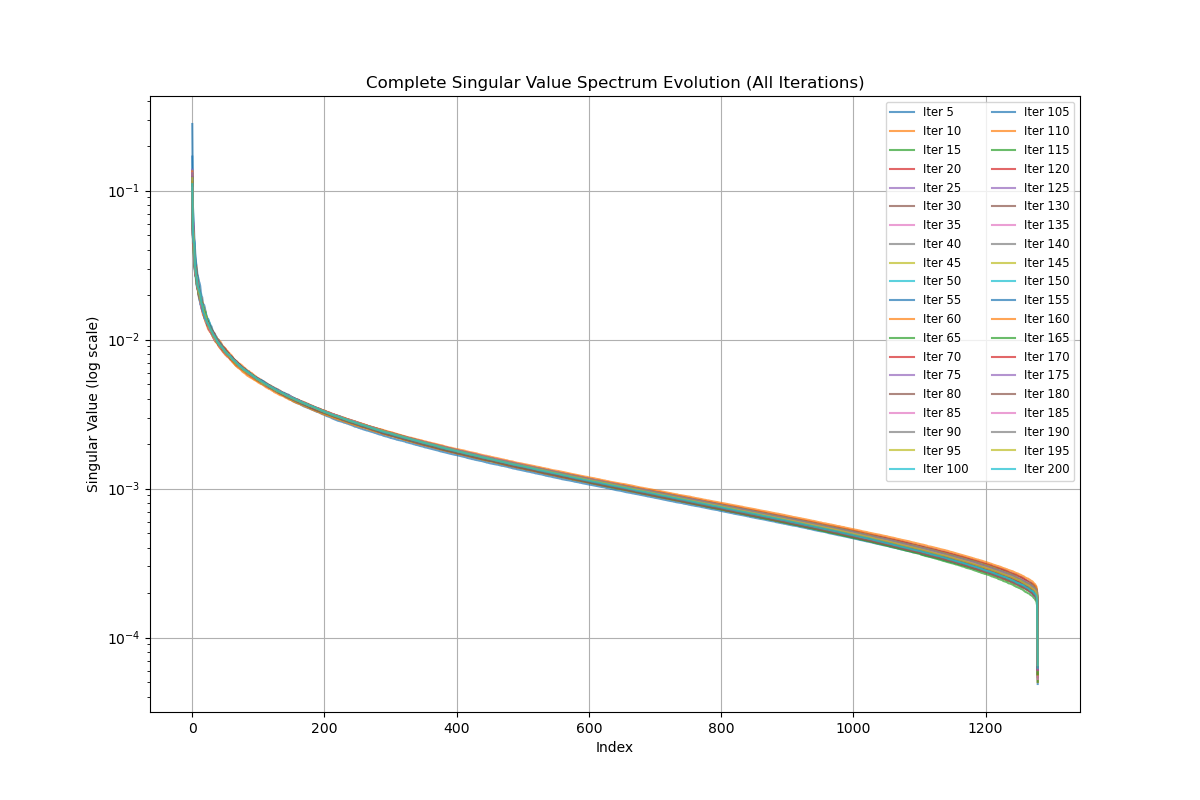
\includegraphics[width=0.8\linewidth]{figs/mlp24/svd_evolution_all.png}}
        \caption{Singular values of $50257\times 1280$ layer via 200 iterations}
        \label{fig:svd_all}
    \end{figure}
    \begin{figure}[h!]
        \center{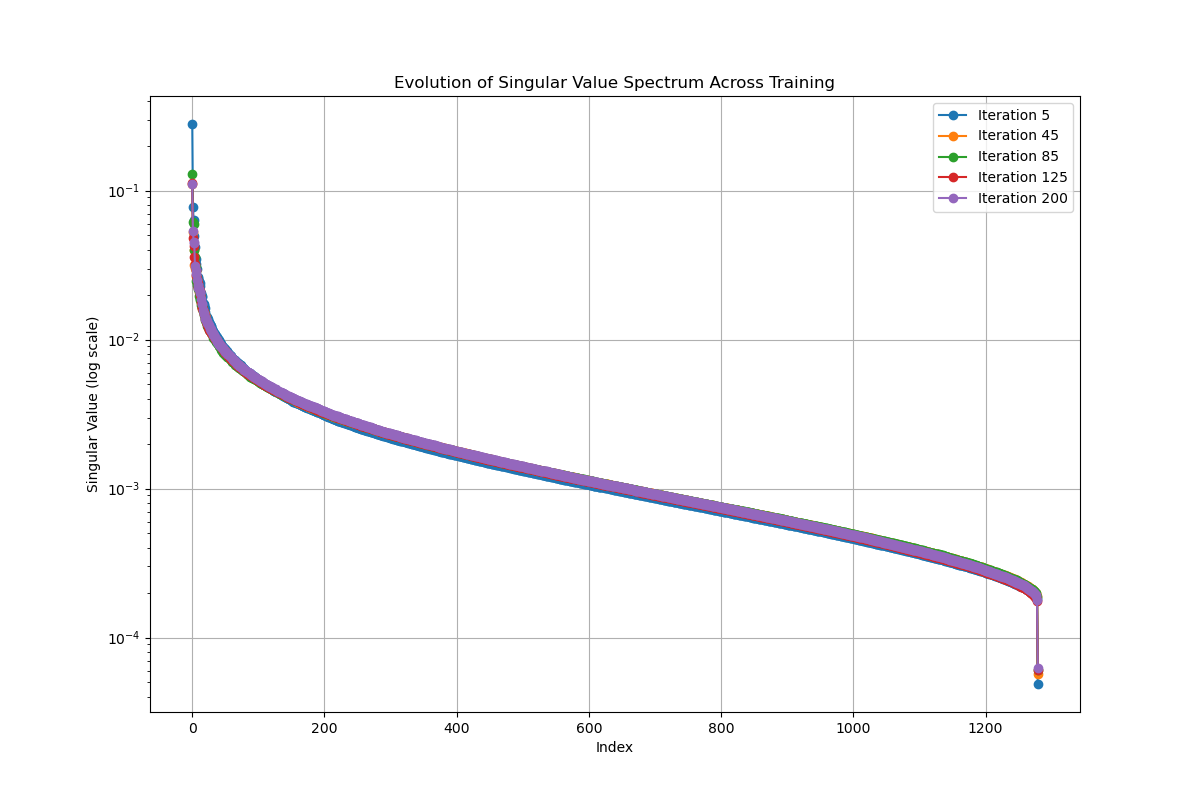
\includegraphics[width=0.8\linewidth]{figs/mlp24/svd_evolution.png}}
        \caption{Singular values of  of $50257\times 1280$ layer for 5-th,45-th, 65-th,175-th and 200-th iteration}
        \label{fig:svd}
    \end{figure} 
    
    \item NanoGPT is tested on Muon and Adam. For now, Neon (rank-1 version) does not converge (see Figures ~\ref{fig:train_loss} \ref{fig:val_loss})
    \begin{figure}[h!]
        \center{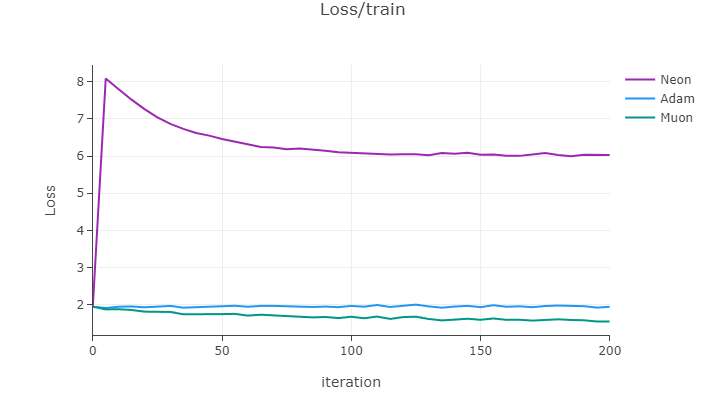
\includegraphics[width=0.8\linewidth]{figs/mlp24/loss_train.png}}
        \caption{Train loss}
        \label{fig:train_loss}
    \end{figure}
    \begin{figure}[h!]
        \center{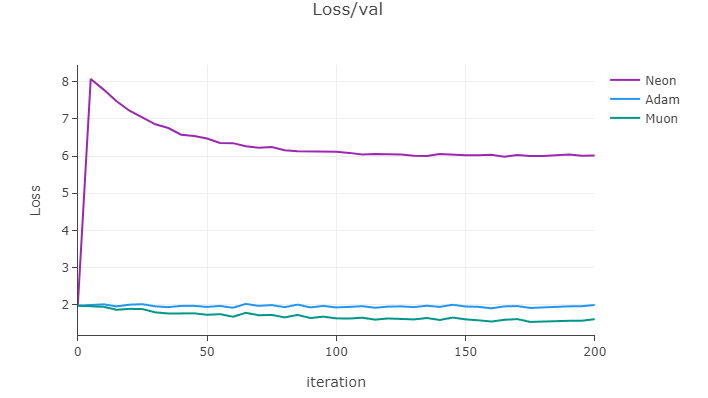
\includegraphics[width=0.8\linewidth]{figs/mlp24/loss_val.png}}
        \caption{Validation loss}
        \label{fig:val_loss}
    \end{figure} 


    The pictures show the best results achieved so far. The experiments were conducted with two 4090 24GB GPUs for nanotgpt-large on the tiny stories dataset.
    
    \item Neon (rank-1 version), Muon, AdamW and SGD are compared on MLP and CNN (see Figures~\ref{fig:mlp_epochs}, \ref{fig:cnn_epochs}, \ref{fig:mlp_time}, and~\ref{fig:cnn_time}). All methods work correctly, but again there is the problem with which one is the fastest (for now, it's SGD).
    \begin{figure}[h!]
        \center{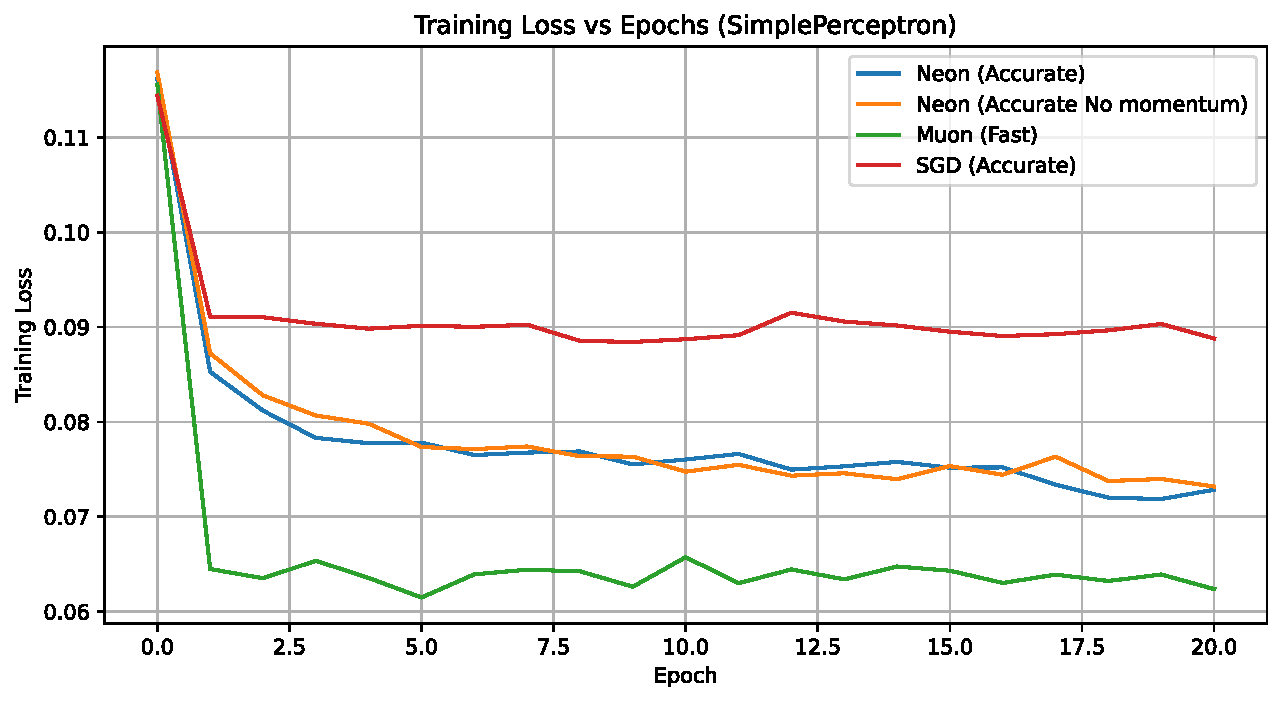
\includegraphics[width=0.8\linewidth]{figs/mlp0605/loss_vs_epochs_mlp.pdf}}
        \caption{MLP: self.linear1 = nn.Linear(32*32*3, 512), self.linear2 = nn.Linear(512, 10), self.activ = nn.GELU()}
        \label{fig:mlp_epochs}
    \end{figure}
    \begin{figure}[h!]
        \center{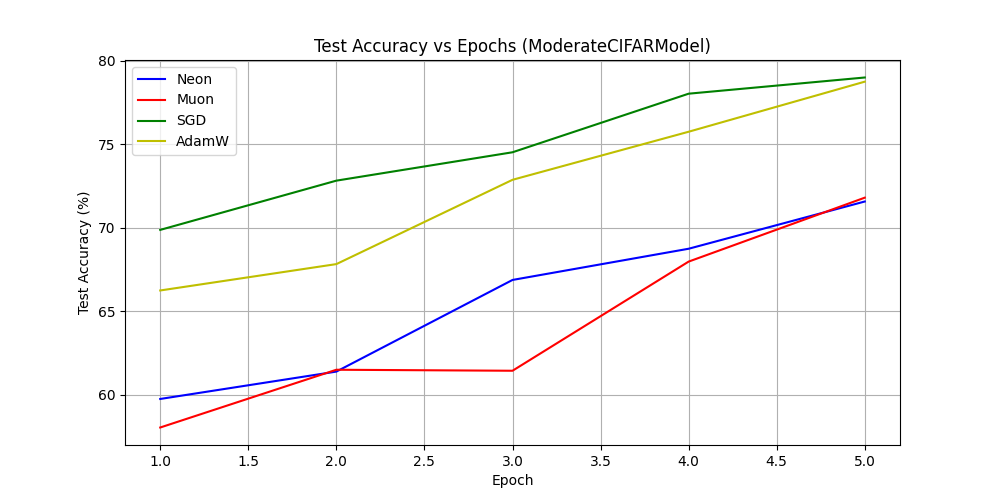
\includegraphics[width=0.8\linewidth]{figs/mlp24/accuracy_vs_epochs_moderate.png}}
        \caption{CNN: 2 convolutional blocks, 2 fully connected layers, activation + dropout}
        \label{fig:cnn_epochs}
    \end{figure}
    \begin{figure}[h!]
        \center{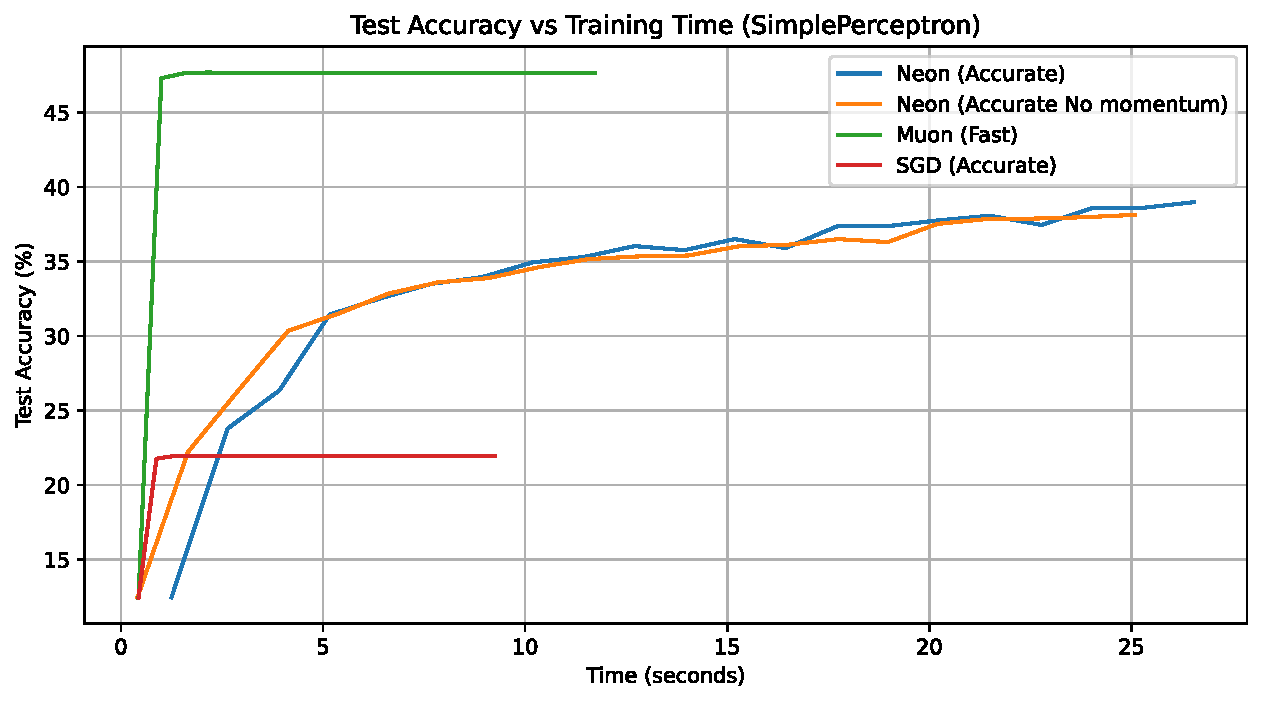
\includegraphics[width=0.8\linewidth]{figs/mlp0605/accuracy_vs_time_mlp.pdf}}
        \caption{MLP: wallclock time measurements}
        \label{fig:mlp_time}
    \end{figure}
    \begin{figure}[h!]
        \center{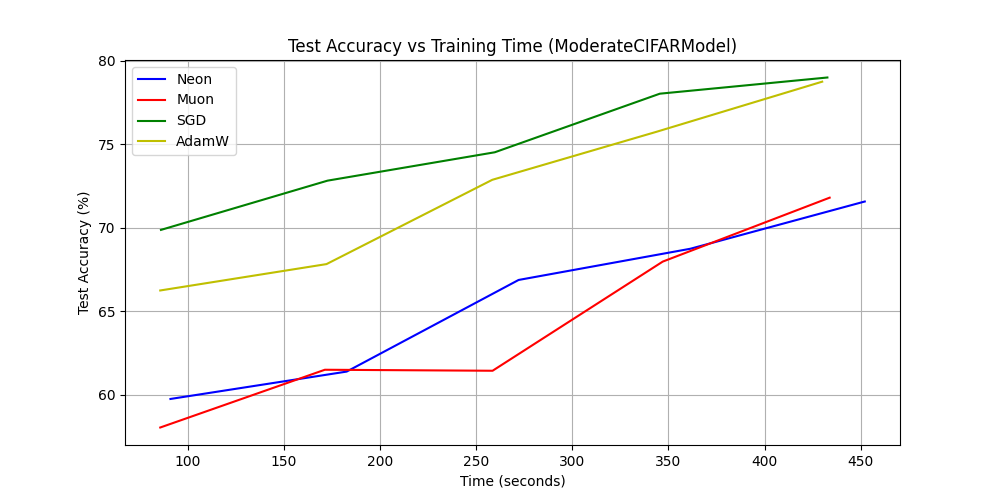
\includegraphics[width=0.8\linewidth]{figs/mlp24/accuracy_vs_time_moderate.png}}
        \caption{CNN: wallclock time measurements}
        \label{fig:cnn_time}
    \end{figure}
    \begin{table}[h!]
        \centering
        \begin{tabular}{c|c|c|c}
        \hline
        Method                              & rtol        & k & time,s \\
        \hline 
        Power Iterations                    & 0.01        & 1 & 7.7\\ 
        SVDS (thick-restart Lanczos method) & 0.01        & 1 & 0.18\\
        PCA Low Rank (RSVD)                 & 0.01        & 1 & 1.15\\
        SVDS (thick-restart Lanczos method) & 0.01        & 10 & 0.47\\
        PCA Low Rank (RSVD)                 & 0.01        & 10 & 19.4\\
        SVDS (thick-restart Lanczos method) & 0.01        & 100 & 1.96\\
        PCA Low Rank (RSVD)                 & 0.01        & 100 & 170\\
        \end{tabular}
        \caption{k-rank updated comparison}
        Comparison of different numerical methods to calculate k-rank update on $5000\times5000$ matrix of real numbers, rtol is an error in Frobenius norm relative to the k-rank approximation of truncated svd. During the research it was noted that rsvd can give good and fast approximation for singular values, but the matrix of approximation is far from the one given by truncated svd, while Lanczos method gives good and fast approximation for a matrix, but not so good approximation for singular values. 
        \label{tab:matrix_methods}
    \end{table}
\end{enumerate}

\bibliography{icomp2024_conference}
\bibliographystyle{icomp2024_conference}

\appendix
\section{Appendix}
You may include other additional sections here.

\end{document}
